Contemporary online multimodal platforms provide an appealing, rich user experience from social media and e-commerce online shopping to crowdfunding. Users may promote or market their ideas, products, or personal brands through a combination of various types of modalities, such as text and images, to attract user attention. However, the properties of effective online multimodal marketing campaigns challenge computational analysis. Potentially, synergy across the multi-sensory information space facilitates faster and more accurate processing to establish semantic relationships \cite{laurienti2004semantic,spence2011crossmodal,wickens2008multiple}, . While the computational modeling of multimodal content has shown advancements, there remains an opportunity for deeper integration of explicit human knowledge, experience, and reasoning. Earlier and smaller (multimodal) Visual Language Models (VLMs) such as MMBT \cite{kiela2020supervised}, ViLBERT \cite{lu2019vilbert}, and LXMERT \cite{tan2019lxmert} primarily focused on exploiting unimodal cues (e.g., textual, visual) to establish connections between image and text. More recent very large VLMs, such as LLaVA \cite{liu2023visual}, BLIP2 \cite{li2023blip} and GPT-4 \cite{openai2023gpt4}, have demonstrated considerable progress in capturing  \emph{implicit} multimodal semantic relationships. However, these models typically operate without semantic constraints, making them vulnerable to hallucinations--- \emph{superficially congruent} \cite{hasanyou,Meyer2022-cf} and  \emph{catastrophically incorrect} \cite{shuster2021retrieval,Maynez2020-cj}. Despite their advancement, these models often remain unable to identify the explicit semantic connections between modalities that are crucial for mirroring human interpretation. \cite{ji2020leveraging}. This limitation can pose challenges while computationally assessing and generating multimodal content for online marketing campaigns, highlighting the need for further enhancement of these models to harness their potential \cite{mcguffie2020radicalization,weidinger2022taxonomy,tamkin2021understanding,de2023chatgpt}. 

Consider the image and text in Figure \ref{fig:image-womens-movement-patriachy}, drawn from our dataset. 
%One can see in the image 
The image contains two women smiling with the saga sign and the text \emph{"Let's Go!"}. The intended holistic meaning can be determined only after seeing the actual caption \emph{"Smash the glass ceiling. Destroy the patriarchy. Save the record store."} The creator of this marketing campaign seemingly intended to promote women's representation in society and the music industry by using an image of two assertive and confident women in the image. The pictured women are, in fact, the unstated subjects of smashing and, as such, destroying male dominance enshrined in patriarchy. Hence, it is crucial to see both modalities and form contextually informed connections to capture the correct meaning of a pair of images and text.

% \vspace{-0.2em}
\begin{figure}[hbt!]
  \centering
  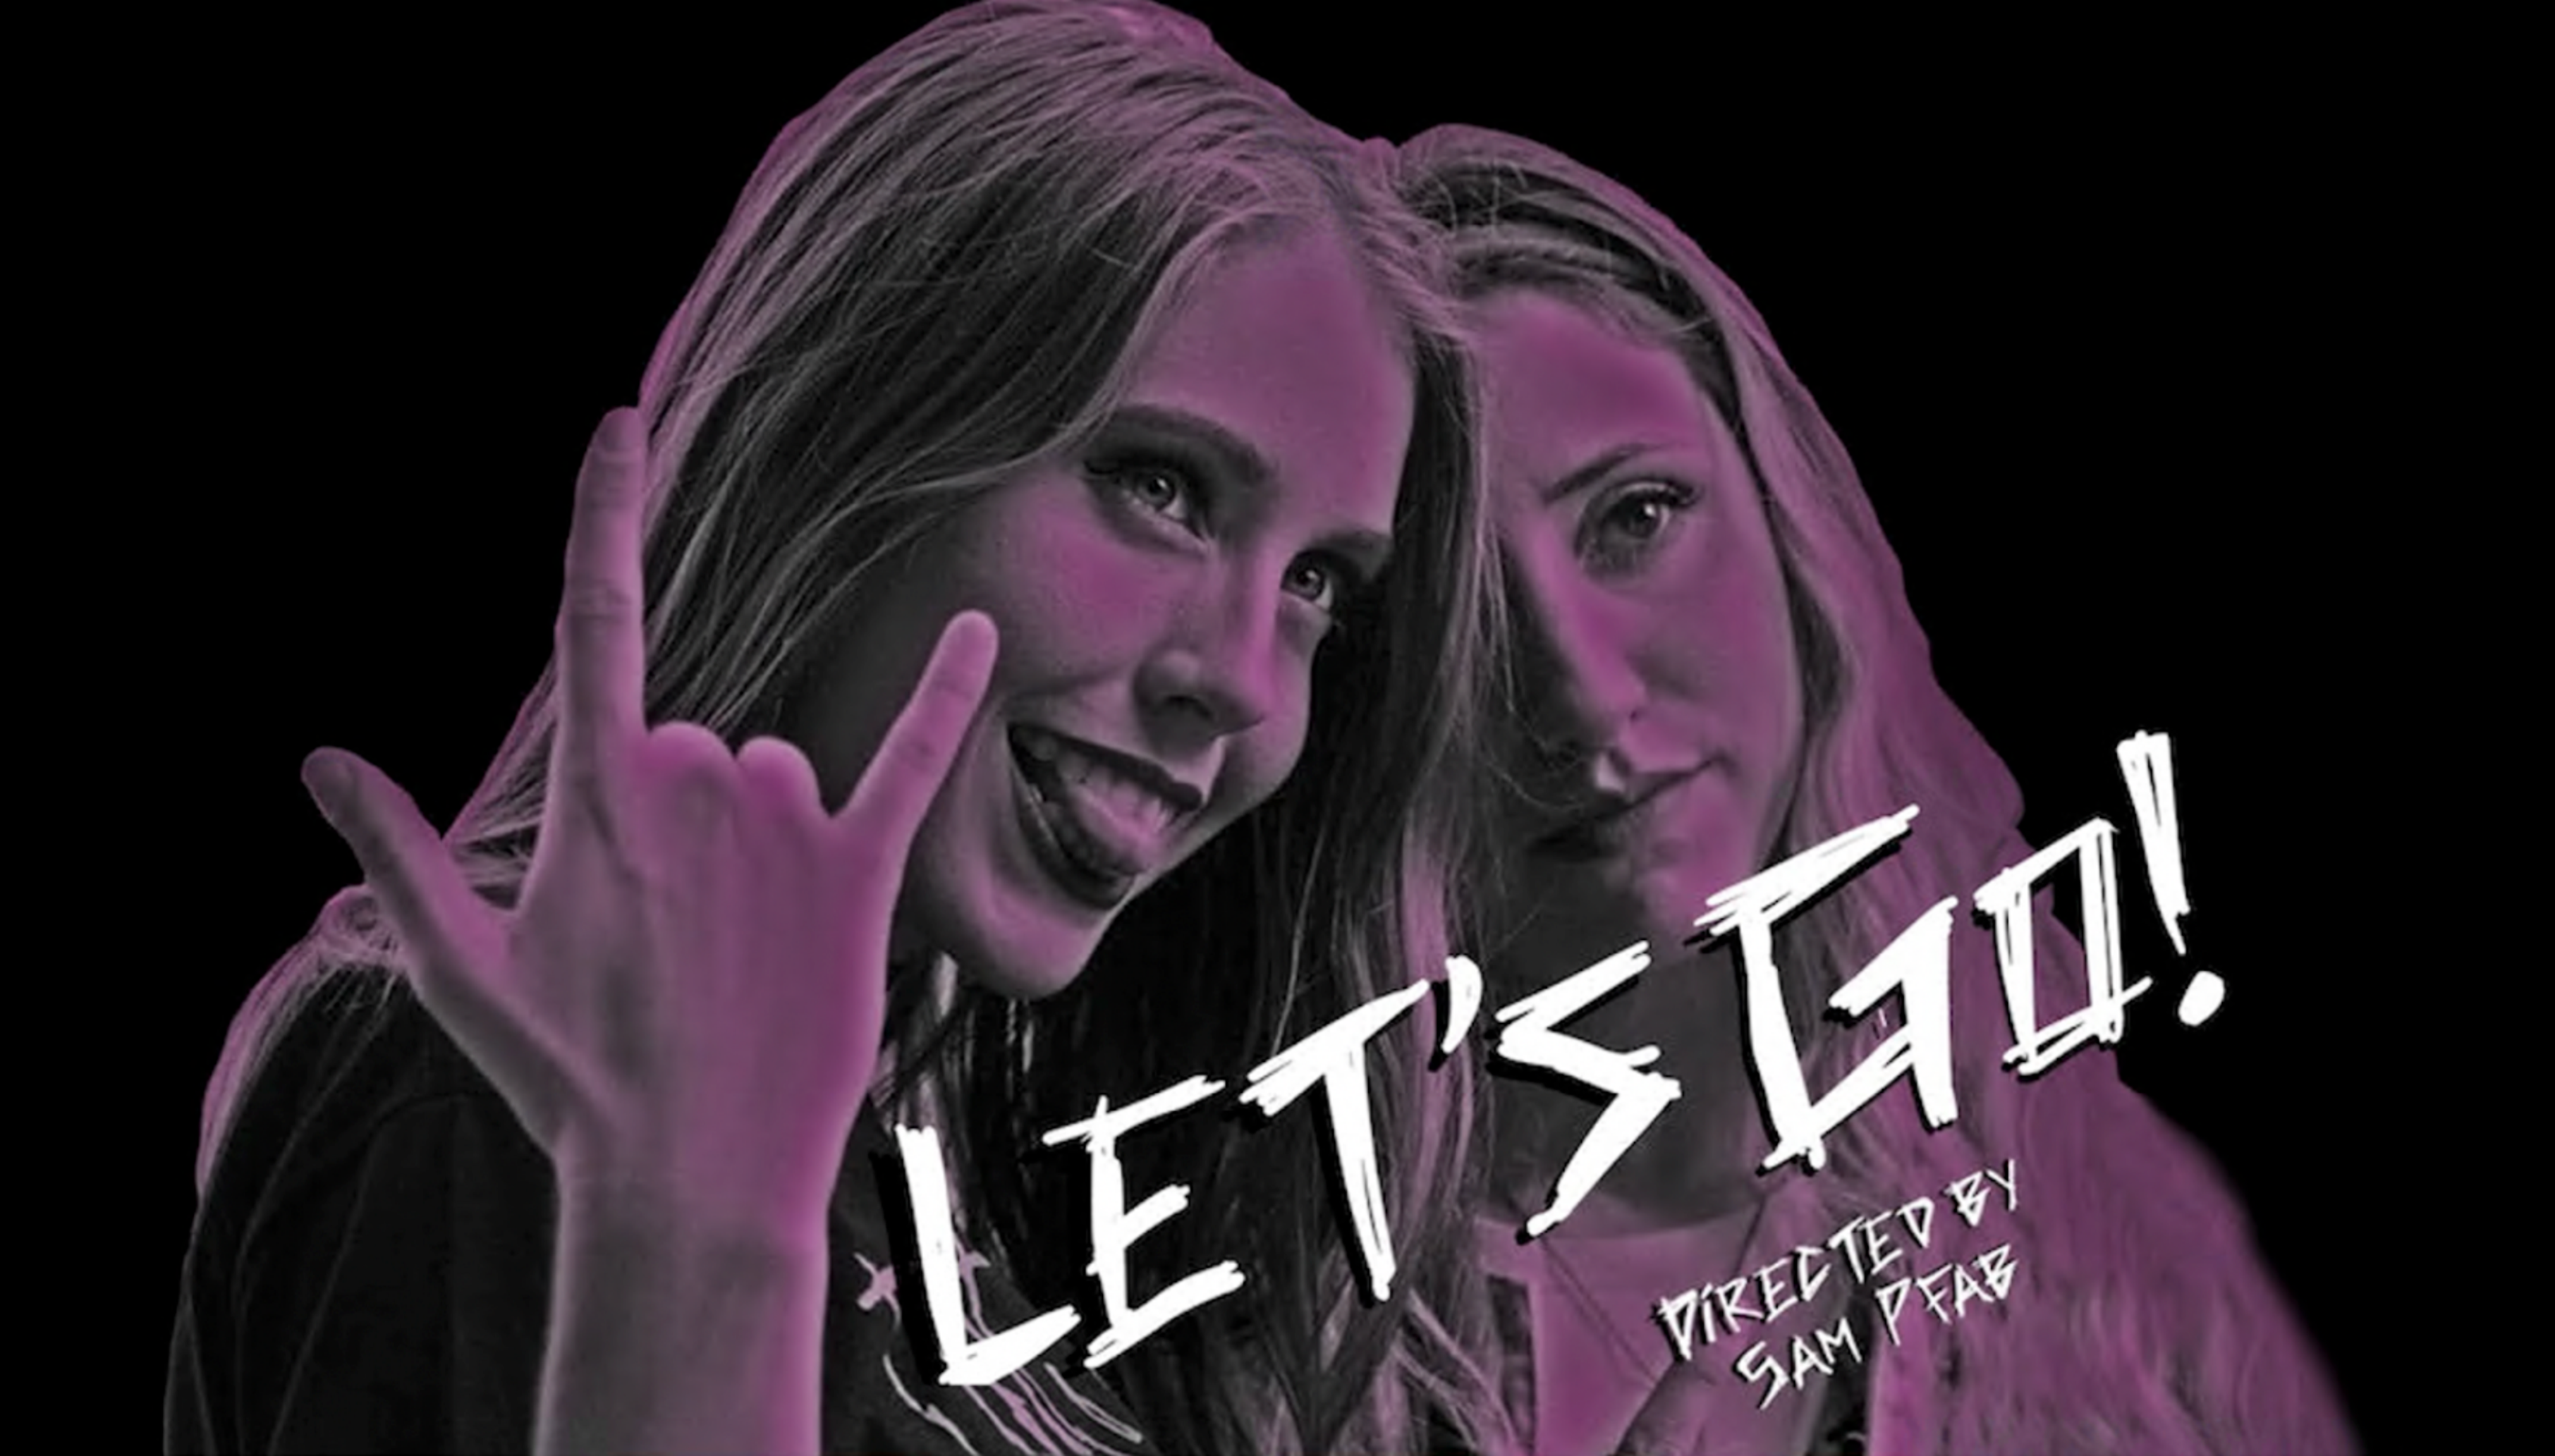
\includegraphics[width=8.5cm]{Figures/record_store_protest-2.pdf}
\vspace{-2em}
\caption{An example pair of image and human caption text from our crowdfunding dataset. The caption generated by the BLIP model and the actual human-generated caption of the image is below. 
\textbf{BLIP caption:} "Two women smiling with a hand gesture of rock and roll." 
\textbf{Actual human caption:} "Smash the glass ceiling. Destroy the patriarchy. Save the record store."}
\vspace{-2.5em}
\label{fig:image-womens-movement-patriachy}
\end{figure} 

Table \ref{tab:generated-caption-two-women} presents explanations generated by state-of-the-art multimodal models, including BLIP2 and LLaVA. While LLaVA \cite{liu2023visual} did generate contextually informed explanations of the input pair, it produced hallucinations, such as describing, “The image features two women standing next to each other, \emph{both holding their cell phones in their hands. They seem to be taking selfies},” when, in fact, there are no cell phones visible in the given image, nor are they taking selfies. To address this issue, we appended the input pairs in our dataset with the most relevant concepts from ConceptNet {\cite{speer2018conceptnet}}. This augmentation mitigated hallucinations as demonstrated in the generated outputs from example pairs in Table \ref{tab:generated-caption-two-women} in Appendix). This comparison highlights the value of multimodal analysis guided by external knowledge, which helps form more accurate cross-modal contextual connections. 

In this study, we examine the following two research questions: \\
\textbf{RQ1:} Can we enhance the cross-modal contextual congruence of the representations of multimodal content by incorporating external knowledge by learning to unveil subtle cross-modal semantic relationships? \\
\textbf{RQ2:} Do more contextually congruent representations help the models obtain more consistent and reliable predictive performance for the success of multimodal crowdfunding campaigns? 

Our work focuses on enhancing the cross-modal contextual congruence of representations of multimodal content for crowdfunding campaigns by incorporating an external Knowledge Graph (KG) (e.g., ConceptNet). As contextual congruence is defined as the association between multiple cues from various modalities (see Section \ref{sec:prelim}), we use ConceptNet, a commonsense knowledge graph with rich semantic knowledge of the world, to synthesize these diverse multimodal cues similarly that mirror human cognitive processes. We first take pairs of images and text from our dataset and generate embeddings using text and image encoders (i.e., via LLMs, LVMs). We generate captions for images to query the KG using BLIP \cite{li2022blip}. Then, our approach retrieves the most relevant concepts from ConceptNet based on semantic search. We learn knowledge graph embedding (KGE) models to generate representations of the resulting concepts. Initially, we learn multimodal data representations using bidirectional transformers. These representations are then fused with the KGEs through a fusion mechanism with linear and multi-head cross-attention layers to obtain enhanced knowledge-infused multimodal representations. 



Our findings indicate that knowledge-infused multimodal representations consistently outperform baseline models without knowledge. Further, we found that augmenting knowledge in the input of multimodal models bridges the semantic gap between the modalities, enhancing the congruence by bringing them closer. Error analysis (see \ref{sec:results-discuss} Section Results \& Discussion) reveals how external knowledge improves the capture of intended holistic multi-modal meaning. We demonstrate the contribution of knowledge to machine learning algorithms for computational analysis of crowdfunding campaigns, which provide an ecologically valid measure of success.

The contributions of this work lie in modeling a social and behavioral problem, such as successful crowdfunding campaigns, utilizing neural and symbolic models \cite{sap2022neural}. In so doing, we particularly tackle the problem of learning a contextually enhanced neural representation of multimodal content with external commonsense KG (i.e., symbolic) \cite{yu2022probabilistic}. This helps the model to better capture the holistic meaning across modalities, consequently improving the performance in predicting the success of multimodal marketing campaigns.

\begin{table*}[hbt!]
\vspace{-0.2em}
  \centerline{
    \begin{tabular}{p{0.8cm}p{1.3cm}p{14.6cm}}
    \toprule[2pt]
   \textbf{\centering Model} & \textbf{\centering Knowledge} & \textbf{Text Caption} \\
    \toprule[1pt]
    BLIP2 & \centering No & the cover of let's go with two girls posing in front of a purple background going for a protest. \\
    \toprule[1pt]
    BLIP2 & \centering Yes & The cover of a movie "let's go" talks about patriarchy in the record store. \\ 
    \toprule[1pt]
    LLaVA & \centering No & The image features two women standing next to each other, both holding their cell phones in their hands. They seem to be taking selfies or sharing a moment together. One of the women is making a funny face, adding a playful vibe to the picture. The other woman is simply enjoying the moment and being part of the fun. \\ 
    \toprule[1pt]
    LLaVA & \centering Yes & The image features two beautiful and majestic black women standing together, united in their quest to smash the glass ceiling and destroy the patriarchy. They are surrounded by record albums, highlighting their shared passion for music and the record store. Their powerful presence and determination to save the record store from any threat make for a compelling scene that showcases their strength and resilience in the face of oppressive societal norms. \\
    \bottomrule[2pt]
    \end{tabular}%
  }
% \vspace{-0.5em}
\caption{For the image and text pair (see Figure \ref{fig:image-womens-movement-patriachy}), the captions generated by the models BLIP2 and LLaVA when the model was prompted with the Image and Text with and without external Knowledge. The knowledge is extracted from ConceptNet as explained in section \ref{sec:explicit-knowledge} and appended to the prompt input to these models. 
%While t
\emph{The captions with generated knowledge show less hallucination.} See Table \ref{tab:generated-captions} in the Appendix for more examples.}
\label{tab:generated-caption-two-women}
\vspace{-2.5em}
\end{table*}